% Chapter Template

\chapter{Implementation 10} % Main chapter title

\label{Chapter3} % For referencing the chapter elsewhere, use \ref{Chapter1} 

After introducing the project, we will now talk about our implementation.
We tried to keep our architecture loosely coupled, so that the e.g. the communication to Unity would work even if a connection to the webserver failed.
Our implementation used the aforementioned tools as well as some smaller libaries that will be explained in the following section.
\section{Prototyping}
Our reasearch inspired us to try Rapid Prototyping in our project. 
We designed a Proof of Concept for each stage \ref{fig:PoC} of our implementation.
\begin{figure}[th]
	\centering
	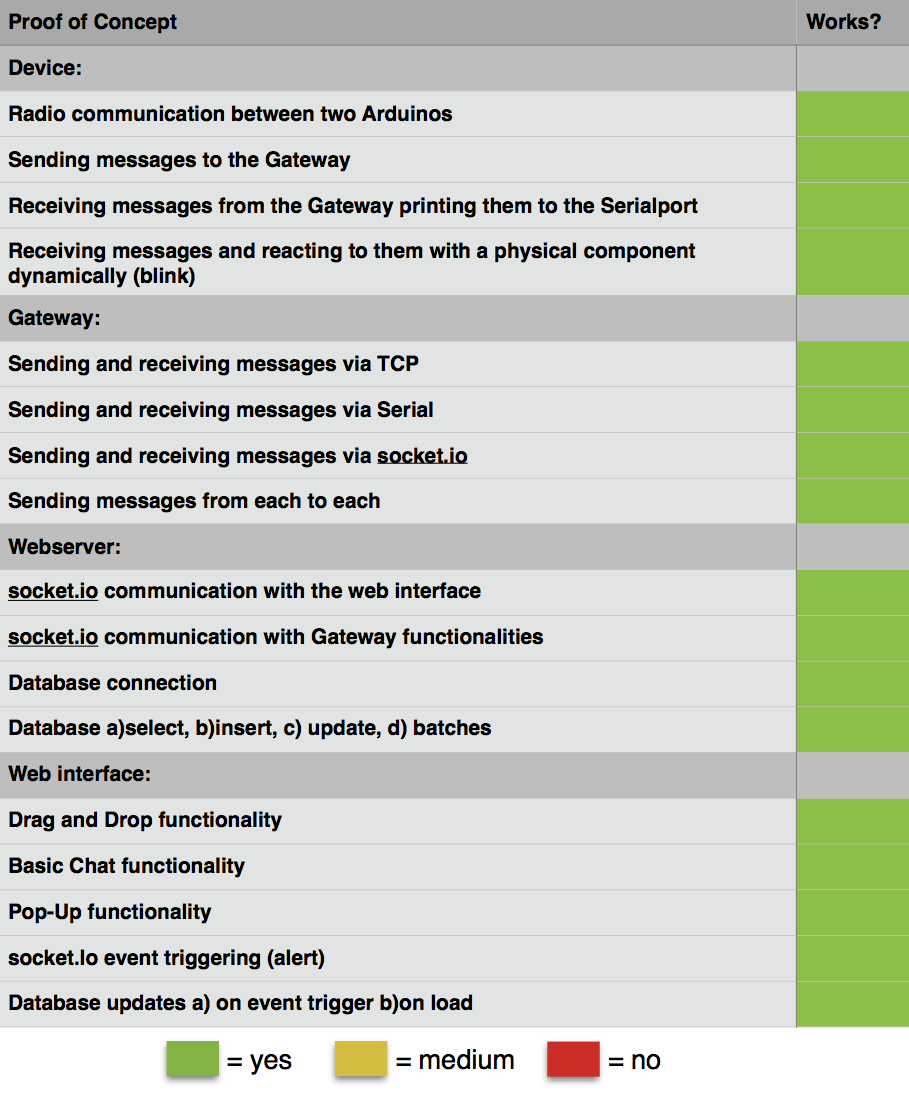
\includegraphics[width=100mm,scale=1]{Figures/PoC}
	\decoRule
	\caption[PoC]{List of our PoC steps}
	\label{fig:PoC}
\end{figure}
Our final result is a MVP %Reference abkürzung 
which provides the bare functionalites but lacks in design and more extensive features which we will explain in the evaluation.
\section{Device}
Since the room consisted of Microcontroller-riddles only at the time of this thesis, we decided to design a prototype and a template for integration of future riddles.
%Fig: Arduino verkabelung für prototype
The template was designed to simplify the process of developing a riddle.
The escape room provided in it's prior form no support for new riddle-developers. 
We decided to modify the existing communication protocols for two reasons.
First, we wanted keep them out of the way (as far as possible) for new developers.
Second, our implementation should be compatible with the older riddles as well, therefore needed to follow the same general rules.

The existing communcation protocol followed a "string-to-chararray-send" and "receive-chararray-to-string" structure.
 %Chararrays are smaller than strings hence faster for radio-communication.
The template is devided into 3 parts: "Groundwork", "Riddlefunctionality" and "Remote Functionality". 
The "Groundwork" section should be filled with libaries, variables and definitions. 
The "Riddlefunctionality" section should contain the riddles functionalities seperated from nearly any communication. 
The only communication that needs to be defined here is when the Microcontroller should send messages and which. That is executed by writing a single line command containing the desired string.
If the string is defined in the "registerRiddle()" function in the "Remote Functionality" section, it will be translated in the web interface. 
Likewise should the "Remote Functionality" section contain any remote commands for interaction with the web interface and the server.
The "Remote Functionality" section consists of two functions: 

"registerRiddle()" where strings to be send once on starting the device are defined. 
These strings set the configuration of the variables in the web interface.
To work, they need to follow a specific structure:
\begin{enumerate}
    \item an Index for the riddlevariable (to order the variables)
    \item a "readonly" or "write" command (to make it static or dynamic)
    \item the name of the variable (to translate)
    \item the value of the variable (needs to be converted into a String)
    \item an optional button value (if it was present, a button would show)
\end{enumerate}
That structure is meant to be applieable for any variable. 

\begin{figure}[th]
	\centering
	\includegraphics[width=75mm,scale=0.75]{Figures/registerRiddle}
	\decoRule
	\caption[FrontViewTable]{"registerRiddle" definition in the Arduino}
	\label{fig:FrontViewTable}
\end{figure}


The other function is named "remoteCommand()" and designed to contain processing of incoming messages from the gateway/Pc.
It's connected to the radio functionality further down in the code nevertheless allows the user not to care about how the messages arrive.
The developer is advised to use a "Switch-Case" structure to define his actions in order to keep the messages understandable. 
For any action concerning the defined variables, the case should match the index of the variable.
%fig arduino def

For our prototype, we used an Arduino Uno with a RFM69HCW module, a keypad, and an I2C-display. 
The riddle would be to guess a code and enter it. 
We wanted the code to be changeable to provide different difficulties. 
Moreover would the riddle possess static  "won", "lost", and "reset"-values to track and control the riddle's state.

\section{Back-End}

\subsection{Web server}
It quickly became apperant that our back-end web server would use Node.js due to the reasons mentioned above.
The decisive factor for this decision was that it would be easier to develop and understand a web server programmed in the same language as the front-end.

As we did all website operations client-side, Node.js main operation was the database and handling. 
We used the "pg-promise" libary \parencite{pg-promise} for our database integration with postgres. 
Depending on the event emittet by the web interface, database-queries to select, update or delete could be triggered.
If the gateway emittet a message, a control mechanism would check if the riddle was known and either add a new riddle, update an existing riddle (if new variables where recognized) or translate the incoming data .

With Socket.io, the client would register whether a front-end or another client would register and forward the needed data from the database. 
By namespacing (creating different channels for different clients), we tried to avoid dispensable traffic.
The gateway would receive the changeable ("write") values and send them to the connected riddles.
The front-end would receive the sorted database data in a sorted json fit to the front-ends data-handling.

%Architecture We tried to implement our functionalities as loosely as possibilities, so 
\subsection{TCP/Serial/Socket.IO-Client}
This part of the back-end changed during our developing process. 
Since it had already been implemented in C++, we wanted to recreate the functionalites however rewrite them in a more understandable way. 
Additionaly, we wanted to filter the serial messages on their way to the Unity-application via TCP.
Since the front-end allowed a reassignement of the messages that would trigger an Unityevent, a backend implementation was needed.
We decided to filter the relevant "Finish"-serialmessages through a PostgreSQL-database, which is compatible with loads of languages and frameworks.

Because many developers of our target group were proficient in C\# from Unity development, we first tried to implement the functionalites with a .NET WPF-App.
This proved to be difficult, as it required multi-threading and communication between the threads. Both are well documented at the MSDN \parencite{MSDN}, 
however due to the mass of different techniques it was hard to get an overview. 
The code we created was easier than the C++ code, though not comparable to the readability of the Javascript-code.
It took us roughly a week to implement the desired functionalites. 

At the end of the project, we decided to revisit our C\# code and tried to implement it in Javascript.
The same functionalites took us about 6 hours to implement, though we did by then have intermediate experience in Javascript and started our C\# implementation with Unity-C\#-Knowledge.
In our perception, the Async-capabilities of Node.js showed a tremendous advantage compared to the threading difficulties wie experienced with the .NET project.

\section{Database}
We normalized our database with two tables, one for the riddledetails shown only when the riddle is clicked, and another for listing the general information.
We used the relational model to manage our database. 
In the relational model, related records are linked by a key predicate common to all. 
In our project, we found that two tables fit our needs. 
One table manages the location, name and other general information about the riddle displayed in the main view, 
whereas the other one is responsible for saving and editing the information displayed in the pop-up window. 
This seperation simplifies database changes, clearifying the tasks happening on the Node.js server.
The Node.js server connects the information when sending to the front-end by assigning the details with the riddle's id to the corresponding riddle. 


\begin{figure}[th]
	\centering
	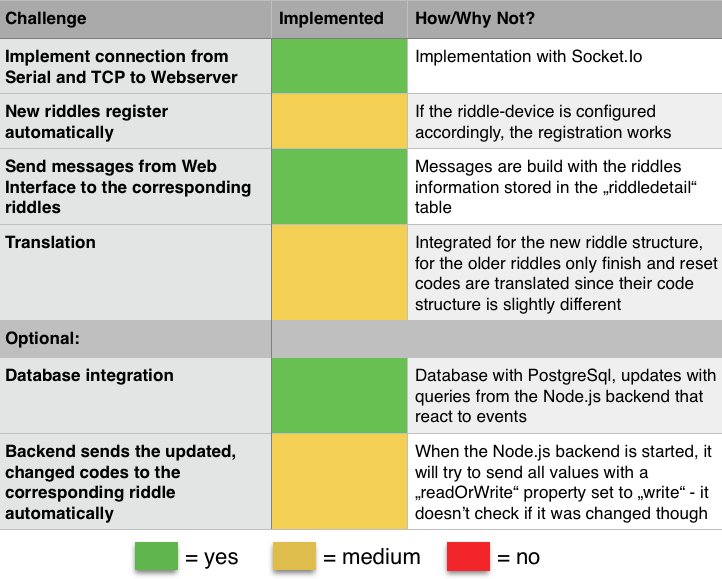
\includegraphics[width=75mm,scale=0.75]{Figures/backendOverview}
	\decoRule
	\caption[FrontViewTable]{Overview about our front-view challenges.}
	\label{fig:FrontViewTable}
\end{figure}

\section{Front-End}
For setting up our front-end, we used the Create-React-App which provides a front-end build pipeline with Babel and Webpack.
React recommends to start there for single-page applications \parencite{createReactApp}. 

It provides a package.json file where you define which version of a module you want to use. This prevents unwanted updates so the code won't risk becoming deprecated.
The npm installer (which is the standard installer for React and Node.js) automatically generates a package-lock.json file which save the dependency tree in further detail.
We discovered GIT-difficulties with the modules and were thankful that we could reinstall the needed packages without having to search which modules we needed.

For our file-structure, we used the recommended approach to group by filetype \parencite{reactStructure} in combination with the Create-React-App-structure.
%Fig: Our File structure front end
Starting out, we wanted to implement a node-editor to connect riddles in all thinkable ways. 
When we listed our wished functionalities (Changeable riddleassignments with "Single", "AND" and "OR" connections to the Unity-Events) we decided that a drag-and-drop table would supply those functionalites (Changeable assignements, OR connections) without creating a difficult User-Interface.
We used the React-dnd libary \parencite{reactDND} to implement the drag-and-drop functionality in React. Currently, it works only on PC since we thought that would be a more popular use case, but adding a mobile implementation for the module is possible.
When a user dropped a riddle into a "Video" field (and saved), the riddle's "Finish"-command would be reassigned on input to the corresponding Video-Trigger-command. 
For example, the "Video1" command was originally triggered by "Riddle1". 
If a user wanted to make "Riddle2" trigger "Video1", he needed to replace "Riddle1" in the "Video1"-List with "Riddle2". 
Whenever "Riddle2" would now signal it's finished, the "Finish"-code of "Riddle1" would be sent to Unity via TCP.

If a Riddle was newly registered, it would be named "NewRiddle" and appear in the "Unassigned Riddles"-List on the web interface.
We designed an "Edit"-function which enabled changing the name of the riddle and deleting it in case it got corrupted (or deleted in real-life).

Another aspect was the popup-window for the riddles. We wanted it to show enough information, yet keep it simple. 
Consequently, our layout for the popup-window was designed flexibly to adapt to a desirable output depending on the usecase:

Each variable would be displayed in respect to it's in the Arduino defined values. 
If a variable was set "readonly", but didn't have a button value defined, the information would be listed plainly.
If a variable was set "write", but didn't have a button value defined, the information would be listed plainly. 
Additionaly, an input field would enable changing the defined value and sending it to the Arduino automatically next time the Server would start. 
If the Arduino was programmed to interpret the incoming value, a variable could be changed that way (e.g. a password in a riddle).
If a button component was set in a variable, a button would appear instead of plain information about the variable. 
The user would be able to click the button to send the code immediately to the riddle. 
This functionality was especially designed with "Finish" and "Start" functionalities in mind, where a supervisor of the escape room might want to trigger these functionalites during a game if customers get stuck.
To increase the general overview for a supervisor, the color of a riddle would change to green once it's "Finish"-code arrived.

\begin{figure}[th]
	\centering
	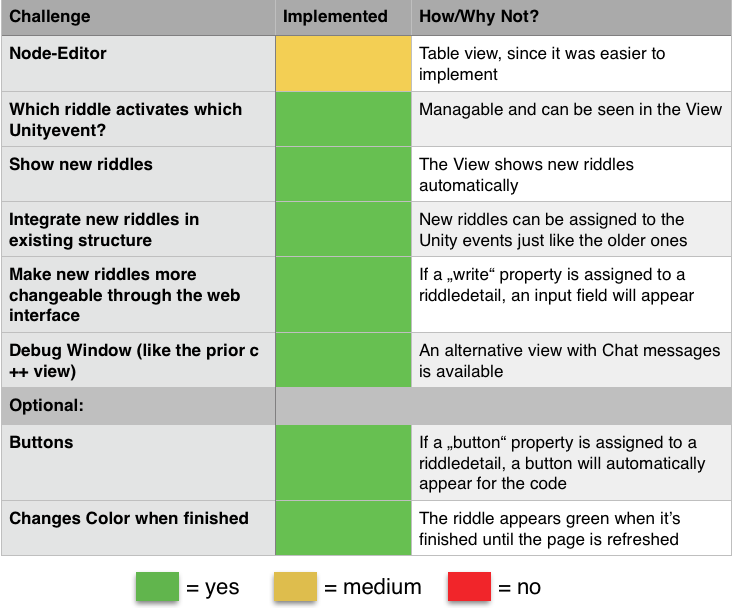
\includegraphics[width=75mm,scale=0.75]{Figures/frontendOverview}
	\decoRule
	\caption[FrontViewTable]{Overview about our front-view challenges.}
	\label{fig:FrontViewTable}
\end{figure}


